\documentclass[
%	draft
	final
]{beamer}
\usepackage{tikz}
\usepackage{subfig}
\usepackage{xspace}
\usepackage{listings}
\lstset{
	language={[11]C++},%
	basicstyle=\ttfamily\small,%
	tabsize=2,%
	keywordstyle=\color{blue!50!black}\fontseries{b}\selectfont,%
	morekeywords={Model,%
		ParticleFactory,%
		HelicityFormalism,%
		BreitWigner,%
		CachedValues,%
		CachedDataValues,%
		DataPoint,%
		DataPartition,%
		Particle,%
		DecayChannel,%
		ParticleFactory,%
		EvtGen,%
		ZemachFormalism,%
		Flatte,%
		Parameter,
		CachedValue,
		CachedDataValue,
	},
%	morekeywords={
%		string,%
%	},% std:: functions
	keywords=[2]{__global__},% CUDA keywords
	keywordstyle=[3]{\color{green!60!blue}\fontseries{b}\selectfont},%
	keywords=[3]{threadIdx},% cuda built-in variables
	keywordstyle=[2]{\color{green!60!red}\fontseries{b}\selectfont},%
%	keywords=[4]{1, 2, 3, 4, 5, 6, 7, 8, 9, 0},%
%    keywordstyle=[4]{\color{green!60!red}\fontseries{b}\selectfont},%
	commentstyle=\color{darkgray!80},%
    stringstyle=\color{orange!50!black},%
	backgroundcolor=\color{cyan!10},%
}
\renewcommand{\sfdefault}{iwona}
\newcommand{\acronym}[1]{{\sc #1}}
\newcommand{\sm}{\acronym{sm}}
\newcommand{\stl}{\acronym{stl}}
\newcommand{\gpu}{\acronym{gpu}}
\newcommand{\cpu}{\acronym{cpu}}
\newcommand{\yap}{\acronym{yap}}
\newcommand{\cuda}{\acronym{cuda}}

% Setup bibliography
\usepackage[
	backend=biber,
]{biblatex}
\usepackage{csquotes}
\addbibresource{backmatter/bibliography.bib}


\title{A lightweight introduction to \cuda}
\author{
	\input{./AUTHORS}
}

\begin{document}

{
	\usebackgroundtemplate{%
		\tikz\node[
			opacity=0.5,
			inner sep=0pt,
		]
		{
			
\includegraphics[
				height=\paperheight,
		width=\paperwidth,%
		%opacity=.2%
		]{fig/logo4.jpg}%
		};
	}

\begin{frame}

	\maketitle
\end{frame}
}

%	
\begin{frame}
	\frametitle{Strategy}
	\begin{enumerate}
		\item Find computationally demanding calls;
			\begin{itemize}
				\item Valgrind/Cachegrind
			\end{itemize}
		\item Evaluate if porting is possible;
		\item Benchmark the ported code;
	\end{enumerate}
\end{frame}


\section{Application scaling}
	
\begin{frame}
	\frametitle{Strong \& Weak Scaling}

	Assume with a fraction $p$ of its code parallelized running on $N$ processors.
	\begin{block}{Strong Scaling}
		Measure of how, for a fixed overall problem size, the time to solution decreases
		\begin{equation}\tag{Amdahl's Law}
			S = \frac{1}{(1-p) + p/N} \le \frac{1}{1-p}.
		\end{equation}
		Increasing $p$ may be more useful than buying new fancy hadrware.
	\end{block}

	\begin{block}{Weak Scaling}
		Measure of how, for a fixed problem size \emph{per processor}, the time to solution changes
		\begin{equation}\tag{Gustafson's Law}
			S = N + (1-p)(1-N) \ge 1.
		\end{equation}
	\end{block}
\end{frame}


\section{What is CUDA}
	\begin{frame}
	\frametitle{The \cuda{} paradigm}
	\cuda{} programming assumes code runs on \emph{two} different platforms, with \emph{two} different memory spaces.
	\begin{block}{Host (\cpu)}
		\begin{itemize}
			\item Pipelines support a limited number of concurrent threads (e.g.~48 on four hex-core processors with Hyper-Threading);
			\item Threads are heavyweight: context switches are expensive.
		\end{itemize}
	\end{block}

	\begin{block}{Device (\gpu, seen as a \emph{coprocessor})}
		\begin{itemize}
			\item Smallest parallel unit (\emph{warp}) comprises 32 threads;
			\item No context switch: separate registers allocated to all active threads.
		\end{itemize}
	\end{block}
\end{frame}


\section{GPU hardware}
	
\begin{frame}
	\frametitle{Architectures}

	\begin{figure}
		\subfloat[][\cpu{} architecture.]{%
			\only<1>{
				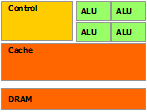
\includegraphics[width=.45\columnwidth]{fig/cpu.png}
			}
			\only<2>{
				
\includegraphics[width=.45\columnwidth]{fig/charlie_cpu.jpg}
			}
		} \quad
		\subfloat[][\gpu{} architecture.]{%
			\only<1>{
				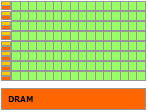
\includegraphics[width=.45\columnwidth]{fig/gpu.png}
			}
			\only<2>{
				
\includegraphics[width=.45\columnwidth]{fig/raymond_gpu.jpg}
			}
		}
	\end{figure}

\end{frame}

	{
	\usebackgroundtemplate{%
		\tikz\node[
			opacity=0.3,
			inner sep=0pt,
		]
		{
			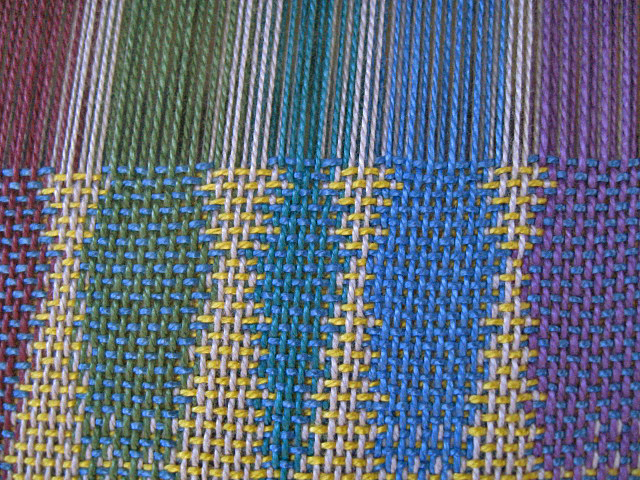
\includegraphics[
				height=\paperheight,
		width=\paperwidth,%
		%opacity=.2%
		]{fig/loom_warp.jpg}%
		};
	}


\begin{frame}
	\frametitle{Hardware implementation}

	\begin{block}{Warps\footnote{``The term \emph{warp} originates from weaving, the first parallel thread technology.''~\cite[p.~69]{cuda:programming}}}
		\begin{itemize}
			\item Are groups of 32 \emph{parallel} threads;
			\item Start at the same program address but each owns an instruction counter and register state so it's free to branch;
			\item Execute \emph{one common instruction at time:} \alert{branches are serialized}.
		\end{itemize}
	\end{block}

	\begin{block}{Streaming Multiprocessors}
		\begin{itemize}
			\item Create, manage, schedule and execute warps;
			\item Run concurrently threads in a block \emph{and} blocks themselves;
			\item Implement no branch prediction nor speculative execution;
			\item \emph{Single Instruction, Multiple Threads:} a single instruction controls all the \cuda{} cores in the multiprocessor.
		\end{itemize}
	\end{block}
%	\gpu{} is built around a scalable array of multithreaded \emph{streaming processors}
\end{frame}
}

%	\input{slides/when_you_actyally_imptove_performances}

\section{Kernels}
	\begin{frame}[fragile]
	\frametitle{The Kernel of \cuda}
	\cuda{} is an extension of C/C++ which allows for \emph{kernels}, functions executed $N$ times in parallel by $N$ different \cuda{} threads.
	\begin{columns}
		\begin{column}{.68\columnwidth}
\begin{lstlisting}
// Kernel definition by means 
// of __global__ keyword
__global__
void VecAdd(float* A, float* B,
            float* C) {
	int i = threadIdx.x;
	C[i] = A[i] + B[i];
}

int main() {
	...
	// Kernel <1 block, N threads> 
	VecAdd<<<1, N>>>(A, B, C);
	...
}
\end{lstlisting}
		\end{column}

		\begin{column}{.32\columnwidth}
			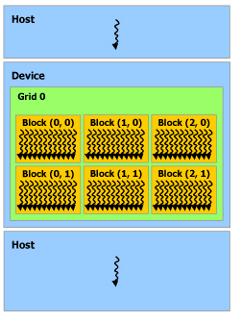
\includegraphics[
				%height=\textheight
				width=1.\columnwidth
				]{fig/heterogeneous-programming_CUT.jpg}
		\end{column}
	\end{columns}

\end{frame}

	\subsection{Threads, blocks \& grids}
	\begin{frame}
	\frametitle{Thread hierarchy}


	\begin{columns}
		\begin{column}{.66\columnwidth}
			\begin{block}{Threads are arranged in \emph{blocks} and}
				\begin{itemize}
					\item
						Can cooperate by sharing data through some per block \emph{shared memory};
					\item
						Can be synchronized with the function \lstinline!__syncthreads()! acting like a barrier.
				\end{itemize}
			\end{block}

			\begin{block}{Blocks are arranged in \emph{grids} and}
				\begin{itemize}
					\item
						Are required to run \emph{independently:} block execution order is \alert{undefined};
					\item
						Are enumerated and distributed to available \emph{streaming multiprocessors} at runtime.

				\end{itemize}
			\end{block}
		\end{column}

		\begin{column}{.34\columnwidth}
			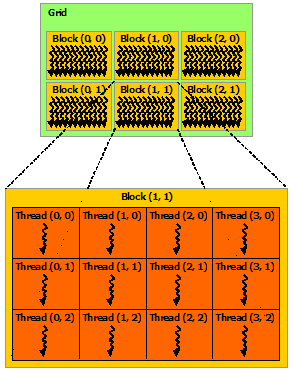
\includegraphics[
				%height=\textheight
				width=1.\columnwidth
				]{fig/thread_hierarchy.png}
		\end{column}
	\end{columns}
\end{frame}


\section{Cuda-based libraries}
	
	\begin{frame}%[fragile]
		\frametitle{\cuda{} out of the box}
			\framesubtitle{\cuda{}-based libraries}
		Some library exist, which are already implemented in \cuda{} and \gpu-optimized such as \lstinline!cuBLAS! (Basic Linear Algebra Subprograms), \lstinline!cuFFT! (Fast Fourier Transform), \lstinline!Thrust!.

		\begin{block}{Thrust}
			\begin{itemize}
				\item C++ template library for \cuda{} based on the \stl{};%~\cite[p.~1]{cuda:thrust};
				\item Manages low level operation such as memory allocation on \gpu{} and copying data between Host and Device;
				\item Provides a large number of common parallel algorithm e.g.~ sortings, transformations reductions.%\lstinline!thrust::sort!, \lstinline!thrust::reduce!
			\end{itemize}
		\end{block}
	\end{frame}


\section{References}
	
\begin{frame}
	\frametitle{References}
	\nocite{*}
	\printbibliography
\end{frame}




\end{document}
